\documentclass[10pt,letterpaper,titlepage]{article}

\usepackage[utf8]{inputenc}
\usepackage[spanish]{babel}
\usepackage{amsmath}
\usepackage{amsfonts}
\usepackage{amssymb}
\usepackage{graphicx}

\author{Gabriel Pérez Mendoza\\
Abraham Toriz Cruz\\
\textbf{Equipo 3}}
\title{Problemas 4 y 5}

\begin{document}

\begin{titlepage}
	\maketitle
\end{titlepage}

\section{Problema 4}

\subsection{inciso a)}

\subsubsection{Problema}
Usando la definición de estabilidad determinar si la solución del siguiente sistema es estable
\[
	3(t-1)\dot{x} = x, \qquad x(2)=0
\]

Primero que nada observamos que este sistema no es autónomo ya que depende explícitamente de $t$, sin embargo podemos hacer algún análisis con los conocimientos obtenidos.

\subsubsection{Solución}
Resolviendo por variables separables

\[
	\begin{array}{rcl}
		3(t-1)\frac{dx}{dt} & = & x\\
		\frac{1}{x} dx & = & \frac{1}{3}\frac{dt}{t-1}\\
		\ln x & = & \frac{1}{3}\ln(t-1) + c_1\\
		x & = & e^{\frac{1}{3}\ln(t-1) + c_1}\\
		& = & c_2 e^{\frac{1}{3}\ln(t-1)}\\
		& = & c_2 \sqrt[3]{t-1}
	\end{array}
\]

Aplicando la condición inicial $x(2)=0$

\[
	\begin{array}{c}
		x(2) = c_2 \sqrt[3]{2-1} = c_2 \cdot 1 = 0\\
		\Downarrow\\
		c_2 = 0
	\end{array}
\]

Quedando la solución como $x(t) = 0$

\subsubsection{Estabilidad del sistema}

Ahora ocupemos la definición de estabilidad para analizar este sistema, pese a que no es independiente la definición no se restringe a algún sistema en particular.

Sea $\epsilon>0$, necesitamos que exista $\delta>0$ tal que si $|x(t_0)-x_0|<\delta$ se cumpla que $|x(t)-x_0|<\epsilon\quad\forall t>t_0$.

Primero tomemos nuestro sistema despejando $\dot{x}$:
\[
	\dot{x} = \frac{x}{3(t-1)}
\]

Esto implica que tenemos un punto de equilibrio en $x=0$, $t \ne 1$.

Aplicando definición de estabilidad obtenemos que:
\[
	\begin{array}{c}
		|x(t)-x_0| = |0-0| = 0 < \epsilon \qquad \forall \epsilon,\\
		|x(t_0)-x_0| = |0-0| = 0 < \delta \qquad \forall \delta
	\end{array}
\]

Así la solución es estable.

\subsection{Inciso b)}

\subsubsection{Problema}
Usando la definición de estabilidad determinar si la solución del siguiente sistema es estable
\[
	\begin{array}{c}
		\dot{x} = -x\\
		\dot{y} = -2y\\
		x(0) = y(0) = 0
	\end{array}
\]

\subsubsection{Solución}

Pasando el sistema de ecuaciones a una forma matricial tenemos:

\[
	\left(\begin{matrix}
		x\\
		y
	\end{matrix}\right)' =
	\left(\begin{matrix}
		-1 & 0 \\
		0 & -2
	\end{matrix}\right)
	\left(\begin{matrix}
		x \\
		y
	\end{matrix}\right)
\]

Dado que es una matriz diagonal $2 \times 2$ podemos saber rápidamente que sus valores propios son

\[
	\begin{array}{rcl}
		\lambda_1 & = & -1 \\
		\lambda_2 & = & -2
	\end{array}
\]

Obteniendo sus vectores propios asociados, para $\lambda_1$ tenemos

\[
	\begin{array}{c}
		\left(\begin{matrix}
			0 & 0 \\
			0 & -1
		\end{matrix}\right)
		\left(\begin{matrix}
			a \\
			b
		\end{matrix}\right) = \left(\begin{matrix}
			0 \\
			0
		\end{matrix}\right) \\
		\downarrow \\
		b = 0 \\
		\downarrow \\
		v_1 = \left(\begin{matrix}
			1 \\
			0
		\end{matrix}\right)
	\end{array}
\]

Ahora para $\lambda_2$ se tiene

\[
	\begin{array}{c}
		\left(\begin{matrix}
			1 & 0 \\
			0 & 0
		\end{matrix}\right)\left(\begin{matrix}
			a \\
			b
		\end{matrix}\right) = \left(\begin{matrix}
			0 \\
			0
		\end{matrix}\right) \\
		\downarrow \\
		a = 0 \\
		\downarrow \\
		v_2 = \left(\begin{matrix}
			0 \\
			1
		\end{matrix}\right)
	\end{array}
\]

Finalmente la solución del sistema quedaría como

\[
	\left(\begin{matrix}
		x \\
		y
	\end{matrix}\right) = c_1 e^{-t}\left(\begin{matrix}
		1 \\
		0
	\end{matrix}\right) + c_2 e^{-2t}\left(\begin{matrix}
		0 \\
		1
	\end{matrix}\right)
\]

luego considerando la condición inicial

\[
	\begin{array}{c}
		\begin{array}{rcl}
			\left(\begin{matrix}
				x \\
				y
			\end{matrix}\right)(0) & = & c_1 e^0 \left(\begin{matrix}
				1 \\
				0
			\end{matrix}\right) + c_2 e^0 \left(\begin{matrix}
				0 \\
				1
			\end{matrix}\right) \\
			& = & c_1 \left(\begin{matrix}
				1 \\
				0
			\end{matrix}\right) + c_2 \left(\begin{matrix}
				0 \\
				1
			\end{matrix}\right)
		\end{array} \\
		\downarrow \\
		c_1 = c_2 = 0
	\end{array}
\]

Si observamos las ecuaciones originales podemos determinar el punto de equilibrio
\[
	\left(\begin{matrix}
		x \\
		y
	\end{matrix}\right)' = 0 \quad\Leftrightarrow\quad \left(\begin{matrix}
		x \\
		y
	\end{matrix}\right) = 0
\]

\subsubsection{Estabilidad de la soluci\'on}

Es digno de observarse que si obtenemos el jacobiano de nuestro sistema de ecuaciones obtenemos la matriz original, debido a que el sistema ya es lineal.
\[
	J = \left(\begin{matrix}
		\frac{\partial (-x)}{\partial x} & \frac{\partial (-x)}{\partial y} \\
		\frac{\partial (-2y)}{\partial x} & \frac{\partial (-2y)}{\partial y}
	\end{matrix}\right) = \left(\begin{matrix}
		-1 & 0 \\
		0 & -2
	\end{matrix}\right)
\]

Finalmente observando los valores propios de la matrix $\lambda_1 = -1$, $\lambda_2 = -2$ podemos decir que puesto que ambos son negativos el único punto de equilibrio debe ser estable.

Más aun, tomando la definición de estabilidad para esta solución observamos que
\[
	|X(t) - X_0| = |0 - 0| < \epsilon \qquad \forall \epsilon>0
\]
y por tanto podemos escoger cualquier $\delta$ que cumpla que
\[
	|X(t_0) - X_0| < \delta
\]
Que de hecho es una $\delta>0$ arbitraria. Luego entonces el sistema es bien estable.

\section{Problema 5}

\subsection{Problema}
Convertir en un sistema de ecuaciones y realizar el estudio completo del sistema restante:
\begin{equation}
x'' + k \sin x = 0 \hspace{20pt} k>0
\end{equation}

\subsection{Solución}

Tomemos el siguiente cambio de variable:
\begin{equation}
	\begin{split}
		y_{1}=x & \Rightarrow y_{1}'=x'=y_{2} \\
		y_{2}=x' & \Rightarrow y_{2}'=x''= -k\sin x
	\end{split}
\end{equation}

As\'i, resulta el siguiente sistema de ecuaciones diferenciales:

\begin{equation}\label{eq:system}
	\begin{split}
		y_{1}' & = y_{2}\\
		y_{2}' & = -k\sin y_{1}
	\end{split}
\end{equation}

Observemos las siguientes propiedades:
\begin{itemize}
	\item El sistema (\ref{eq:system}) es aut\'onomo, ya que NO depende expl\'icitamente de $t$
	\item El sistema (\ref{eq:system}) es no-lineal, ya que en la segunda ecuaci\'on del sistema hay una funci\'on seno que depende de la variable $x$
\end{itemize}

Ceroclinas del sistema (\ref{eq:system}):

\begin{equation}
	\begin{split}
		y_{2} = 0\\
		-k\sin y_{1} = 0
	\end{split}
\end{equation}

Es decir, el conjunto de puntos de equilibrio de (\ref{eq:system}) es el siguiente:
\begin{equation}
	\{(n \pi, 0) | n \in \mathbb{Z}\}
\end{equation}

\subsection{Análisis de estabilidad}
Puesto que el sistema (3) es NO-lineal, tomaremos la matriz jacobiana del sistema y posteriormente evaluaremos los puntos de equilibrio en ella para as\'i saber el comportamiento de la soluci\'on en las regiones alrededor de los puntos de equilibrio.\\\\
La matriz Jacobiana del sistema queda de la siguiente forma:

\[
	J(y_{1},y_{2}) = \begin{pmatrix}
		0 & 1\\
		-k \cos y_{1} & 0
	\end{pmatrix}
\]

Aqu\'i, notamos que tenemos 2 casos a la hora de evaluar: cuando $y_{1}= 2l\pi, l \in \mathbb{Z}$ y $y_{1}= (2l+1)\pi, l \in \mathbb{Z}$\\\\
Caso 1: Evaluando los puntos de equilibrio en J cuando tenemos $y_{1}= 2l\pi, l \in \mathbb{Z}$:

\[
	J((2n) \pi,0) = \begin{pmatrix}
		0 & 1\\
		-k & 0
	\end{pmatrix}
\]

Resultando as\'i el polinomio caracter\'istico de $J$ en:

\begin{equation}
	P(\lambda) = \lambda ^{2} + k
\end{equation}

El polinomio caracter\'istico nos dice que tenemos dos valores propios imaginarios $\pm ki$ (parte real cero), es decir, tenemos centros como se muestra en la figura \ref{fig:orbitas}

\begin{figure}
	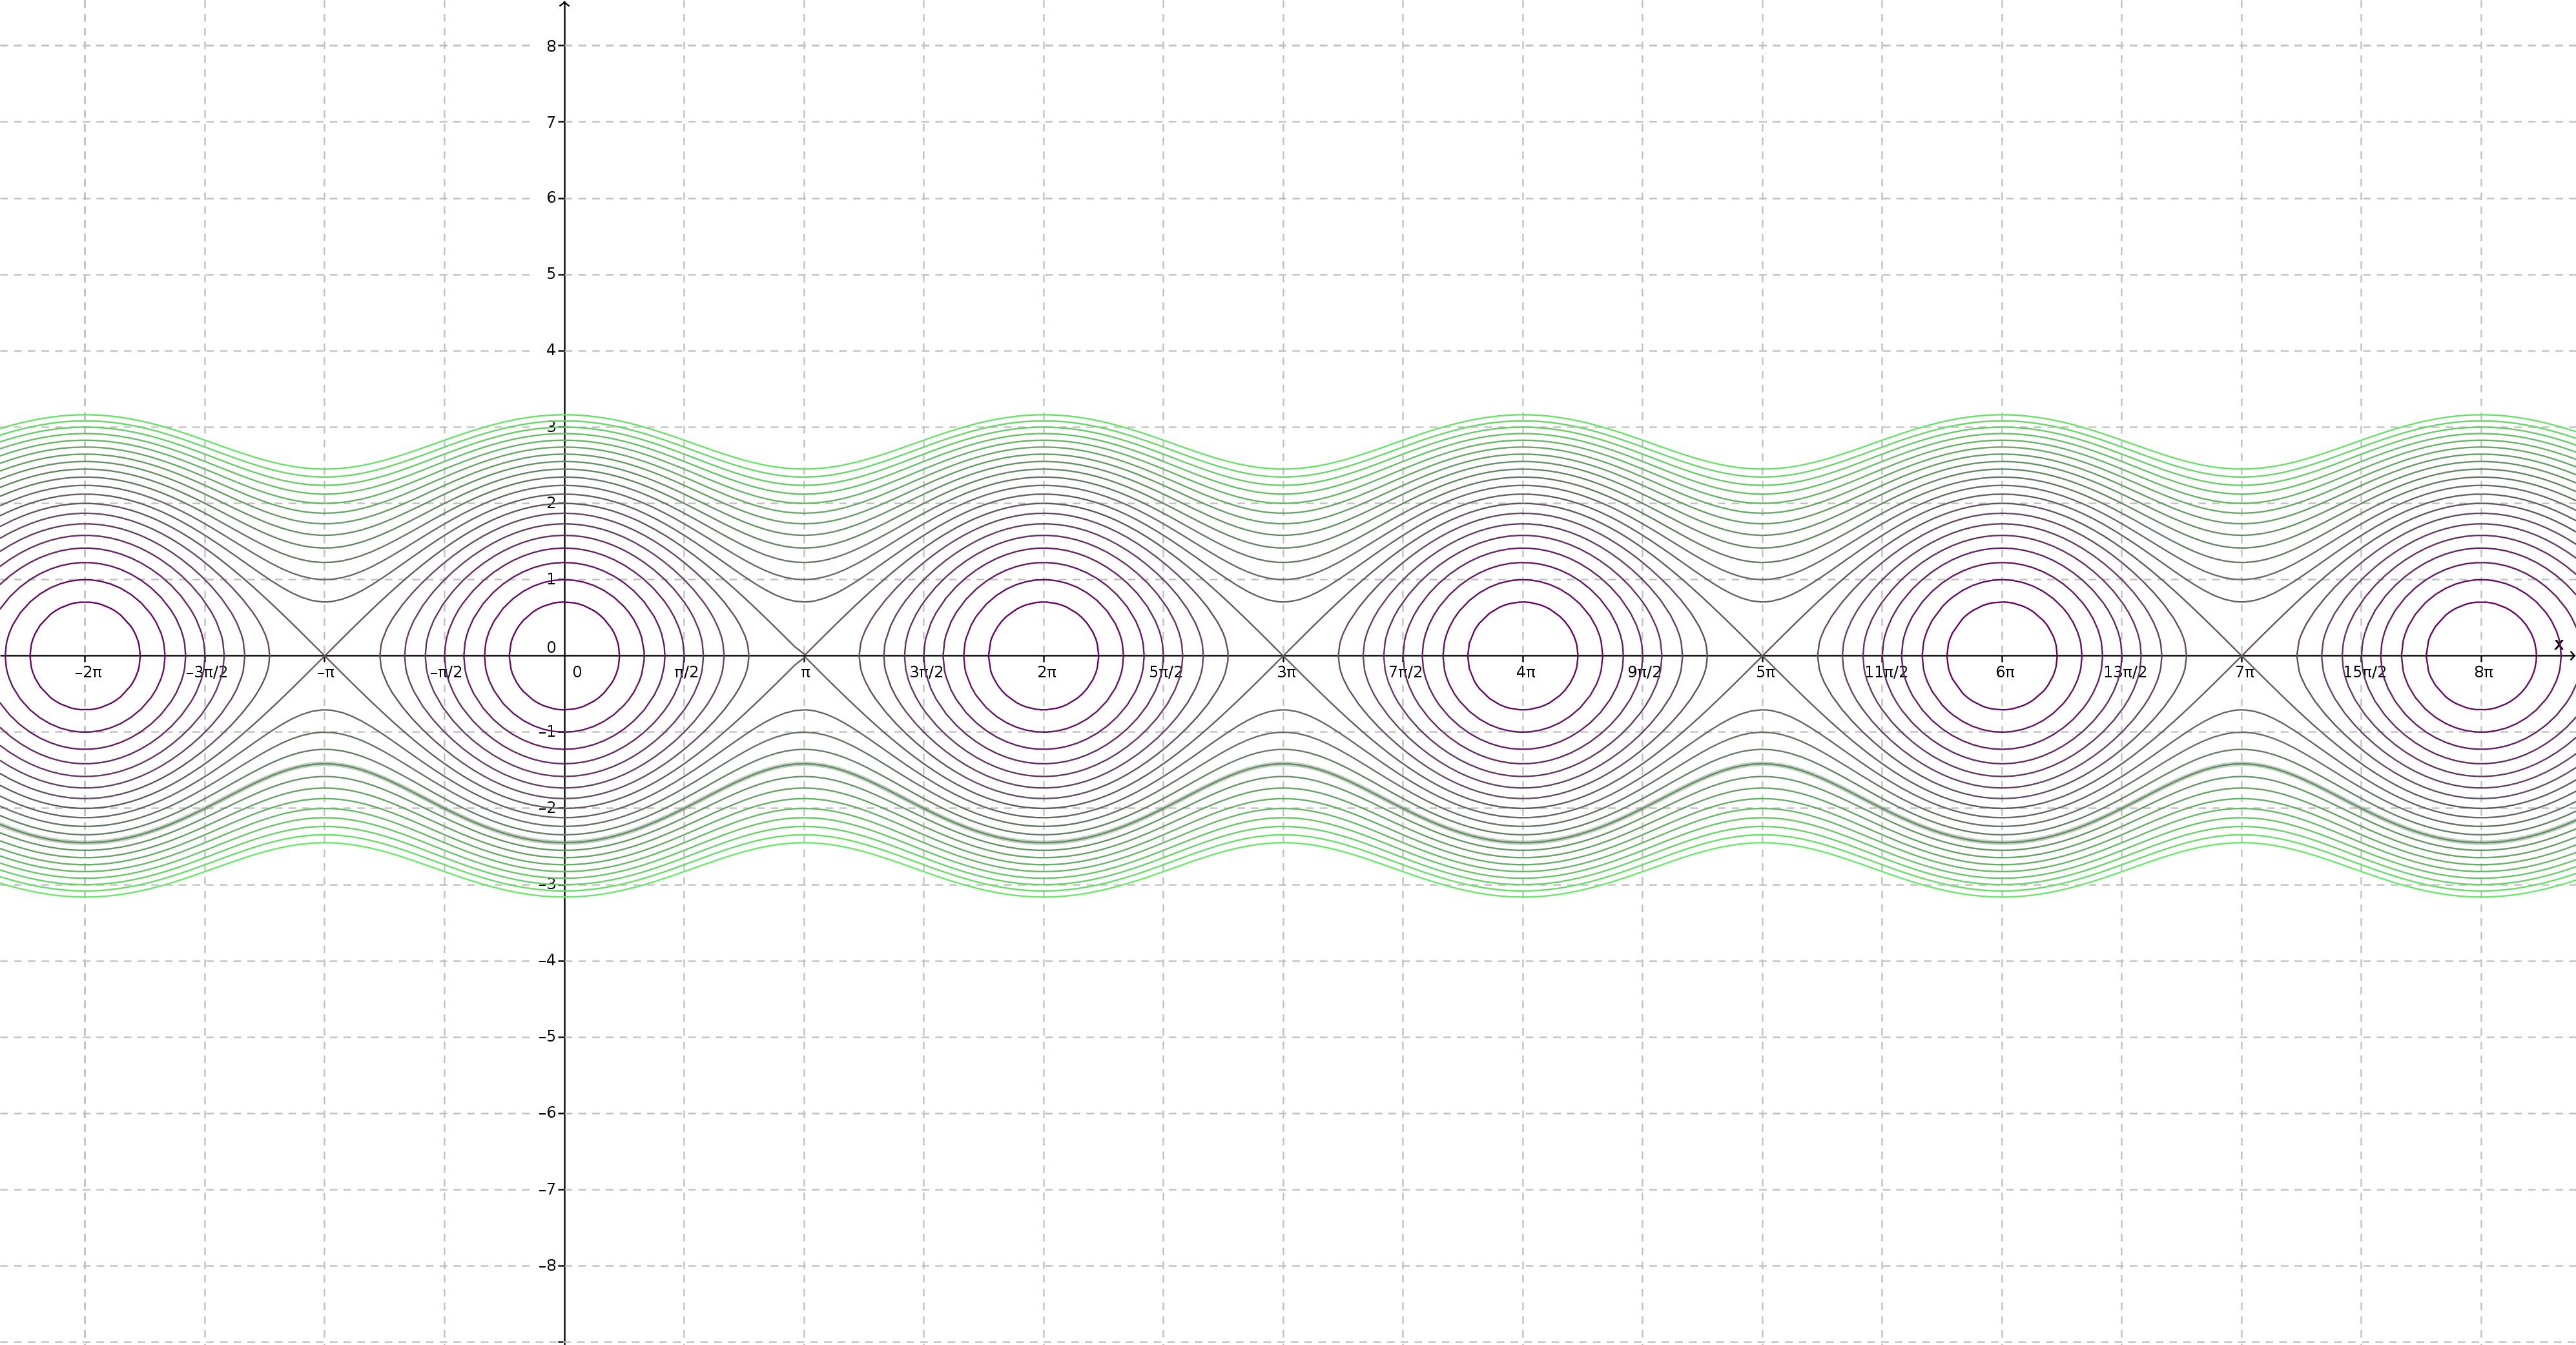
\includegraphics[width=\textwidth]{plot.png}
	\caption{Órbitas alrededor de los puntos de equilibrio con $k=1$}
	\label{fig:orbitas}
\end{figure}

Nótese que si varía el parámetro $k$ de la ecuación tenemos gráficas más alargadas como en la figura \ref{fig:orbitas_largas}.

\begin{figure}
	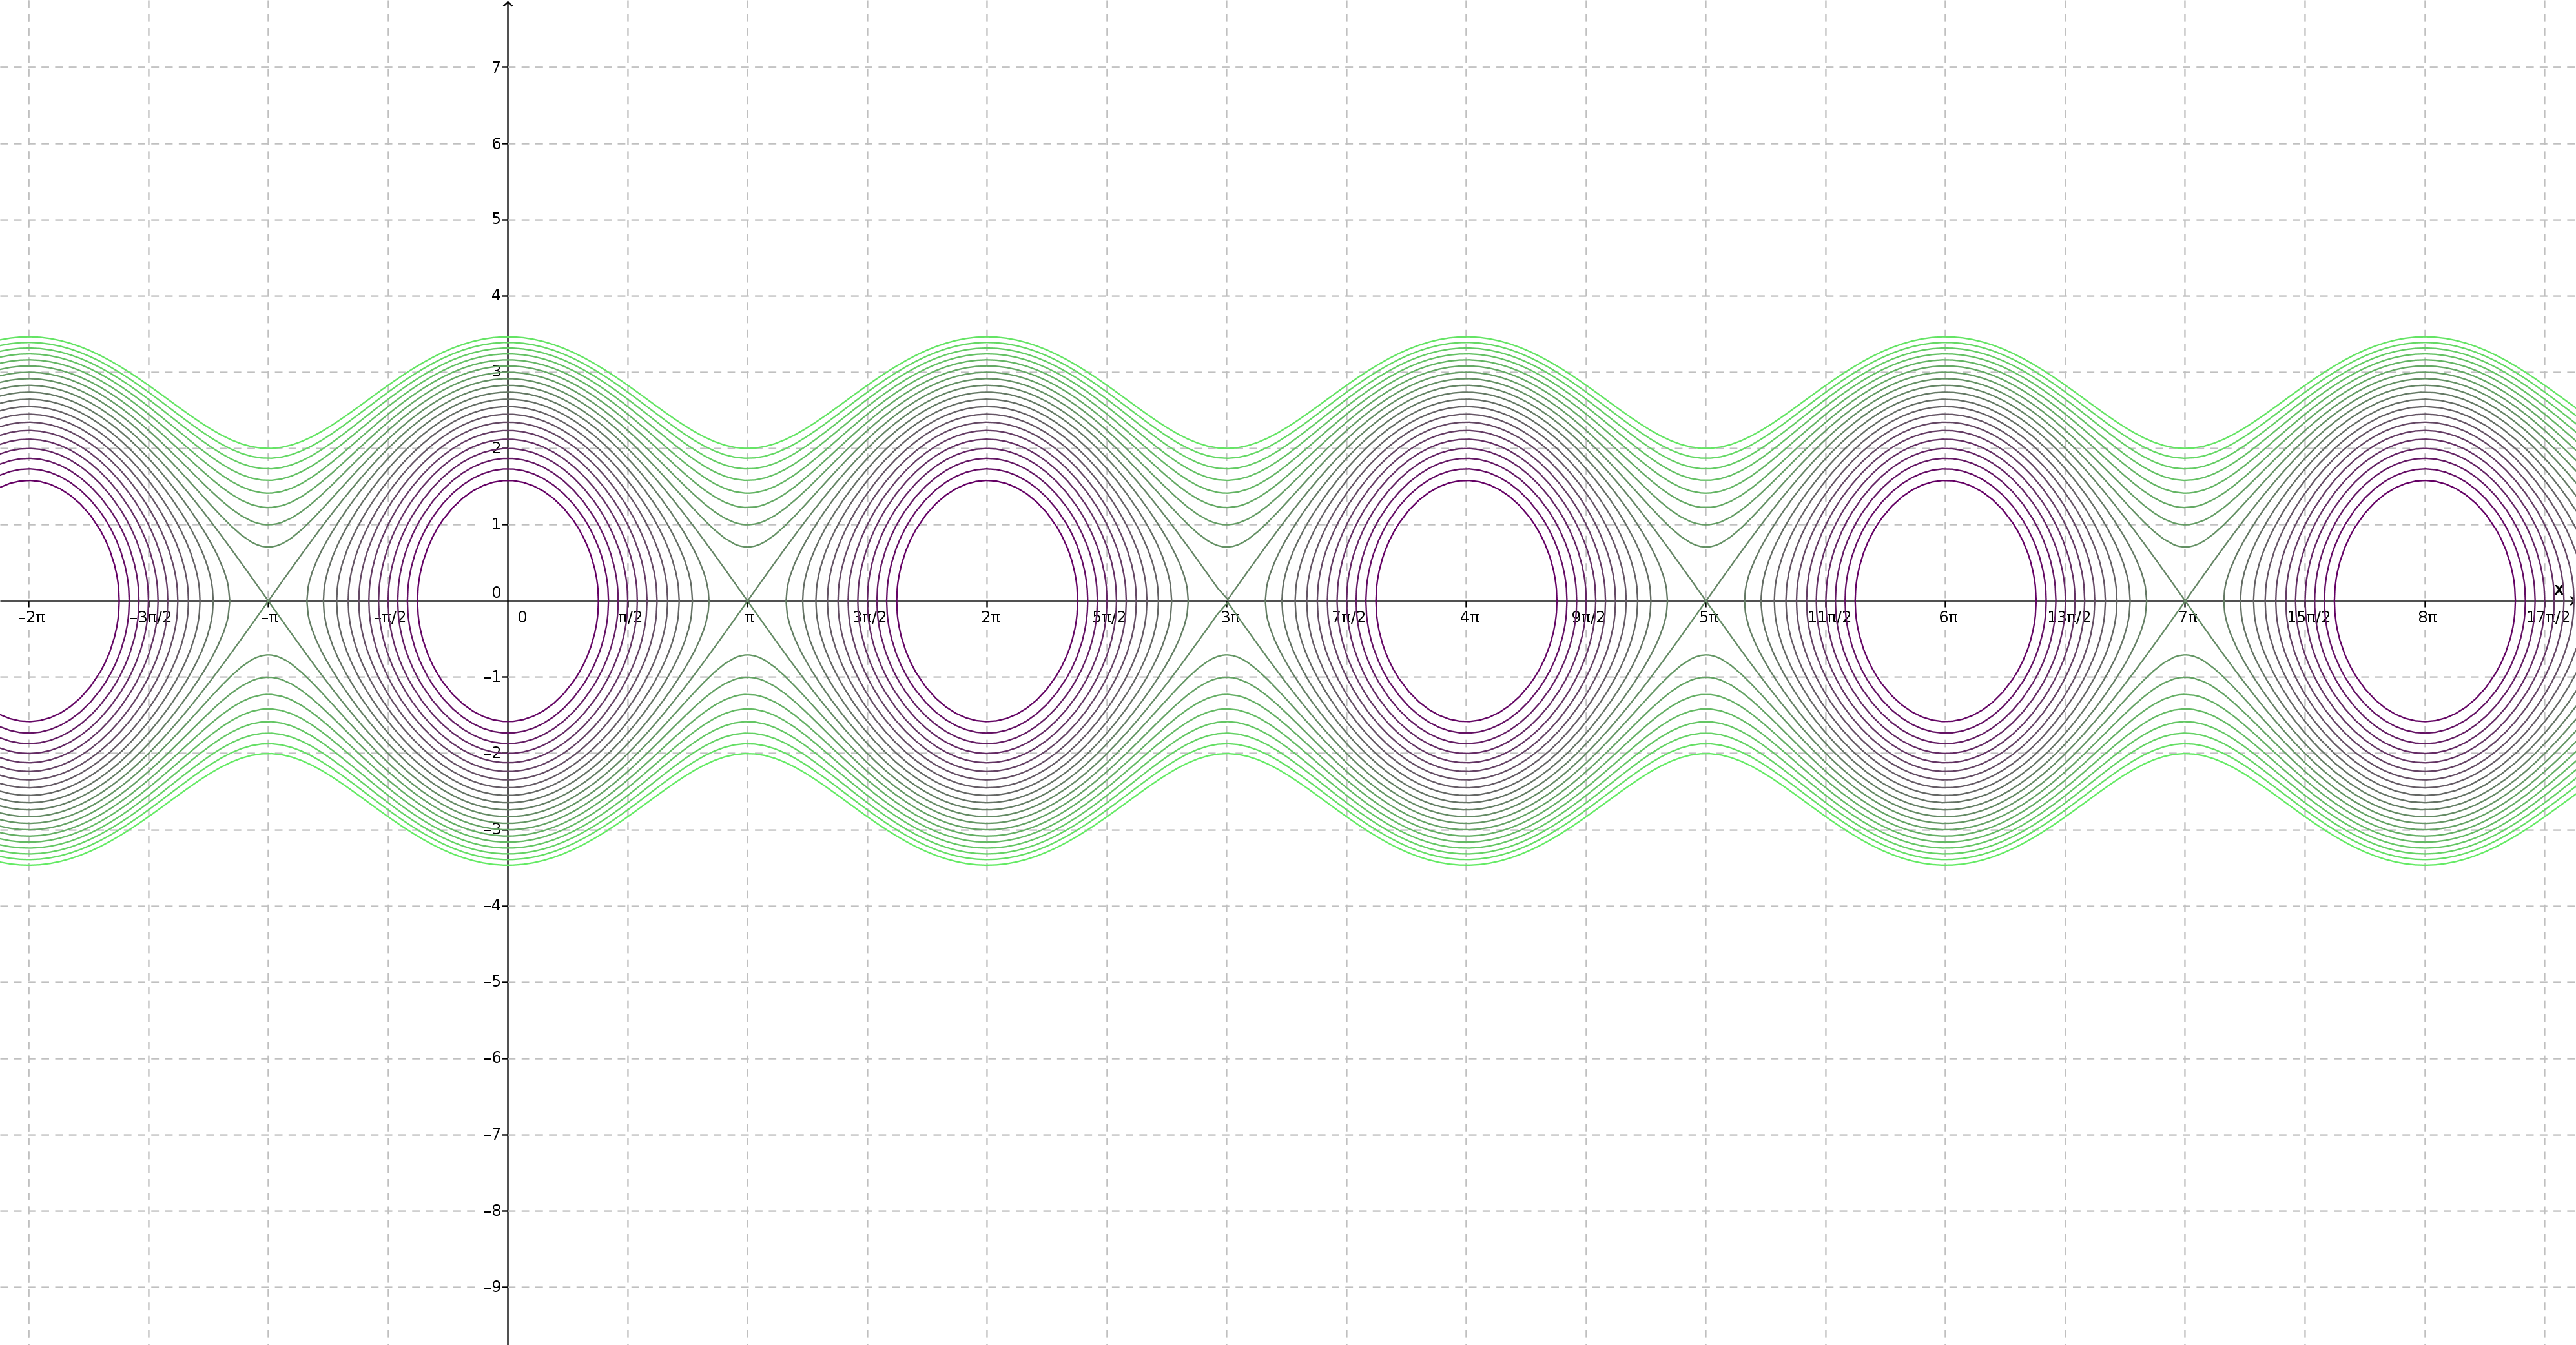
\includegraphics[width=\textwidth]{plot2.png}
	\caption{Variando $k=2$}
	\label{fig:orbitas_largas}
\end{figure}

Caso 2: Evaluando los puntos de equilibrio en J cuando tenemos $y_{1}= (2l+1)\pi, l \in \mathbb{Z}$:
\[
	J((2n) \pi,0) = \begin{pmatrix}
		0 & 1\\
		k & 0
	\end{pmatrix}
\]

Resultando as\'i el polinomio caracter\'istico de $J$ en:

\begin{equation}
	P(\lambda) = \lambda ^{2} - k
\end{equation}

El polinomio caracter\'istico nos dice que tenemos dos valores propios reales $\pm \sqrt{\lambda}$, es decir, tenemos puntos silla.\\\\
Analizamos las regiones alrededor del origen, el cual es un punto de equilibrio(centro) del caso 1:

\begin{itemize}
	\item Regi\'on I: $0<y_{1}< \pi$, $y_{2}>0$.\\
		Como $0<y_{1}< \pi$, entonces $\sin y_{1} > 0$ y as\'i: $y_{2}' <0$.\\
		Como $y_{2}>0$, entonces $y_{1}'>0$.
	\item Regi\'on II: $- \pi<y_{1}< 0$, $y_{2}>0$.\\
		Como $- \pi<y_{1}< 0$, entonces $\sin y_{1} < 0$ y as\'i: $y_{2}' >0$.\\
		Como $y_{2}>0$, entonces $y_{1}'>0$.
	\item Regi\'on III: $- \pi<y_{1}< 0$, $y_{2}<0$.\\
		Como $- \pi<y_{1}< 0$, entonces $\sin y_{1} < 0$ y as\'i: $y_{2}' >0$.\\
		Como $y_{2}<0$, entonces $y_{1}'<0$.
	\item Regi\'on IV: $0<y_{1}< \pi$, $y_{2}<0$.\\
		Como $0<y_{1}< \pi$, entonces $\sin y_{1} > 0$ y as\'i: $y_{2}' <0$.\\
		Como $y_{2}<0$, entonces $y_{1}'<0$.
\end{itemize}

Analizamos ahora las regiones alrededor del punto $(\pi,0)$, el cual es un punto de equilibrio(silla) del caso 2:

\begin{itemize}
	\item Regi\'on I: $\pi<y_{1}< 2\pi$, $y_{2}>0$.\\
		Como $\pi<y_{1}< 2\pi$, entonces $\sin y_{1} < 0$ y as\'i: $y_{2}' >0$.\\
		Como $y_{2}>0$, entonces $y_{1}'>0$.
	\item Regi\'on II: $0<y_{1}< \pi$, $y_{2}>0$.\\
		Como $0<y_{1}< \pi$, entonces $\sin y_{1} > 0$ y as\'i: $y_{2}' <0$.\\
		Como $y_{2}>0$, entonces $y_{1}'>0$.
	\item Regi\'on III: $0<y_{1}< \pi$, $y_{2}<0$.\\
		Como $0<y_{1}< \pi$, entonces $\sin y_{1} > 0$ y as\'i: $y_{2}' <0$.\\
		Como $y_{2}<0$, entonces $y_{1}'<0$.
	\item Regi\'on IV: $\pi<y_{1}< 2\pi$, $y_{2}<0$.\\
		Como $\pi<y_{1}< 2\pi$, entonces $\sin y_{1} < 0$ y as\'i: $y_{2}' >0$.\\
		Como $y_{2}<0$, entonces $y_{1}'<0$.
\end{itemize}

Los resultados anteriores se aprecian en la figura \ref{fig:flujo}

\begin{figure}
	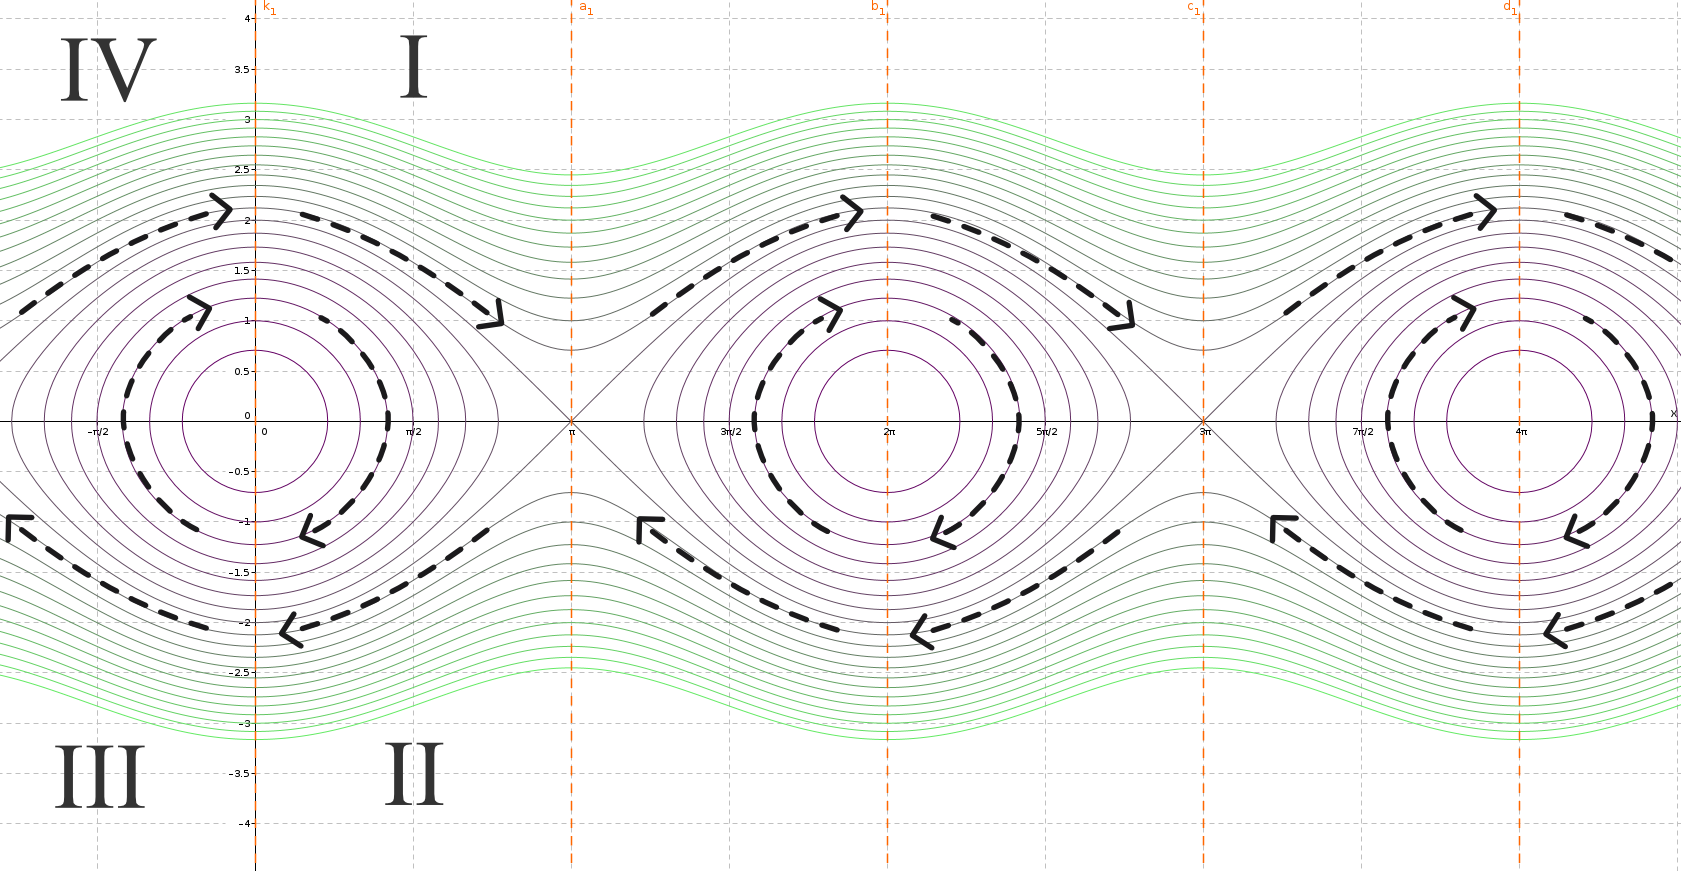
\includegraphics[width=\textwidth]{flujo.png}
	\caption{Flujo de las soluciones}
	\label{fig:flujo}
\end{figure}

\end{document}
